\documentclass[10pt,twocolumn]{article}

\usepackage[letterpaper,top=0.60in,bottom=0.67in,left=0.64in,right=0.64in,columnsep=0.24in]{geometry}
\usepackage[T1]{fontenc}
\usepackage[utf8]{inputenc}
\usepackage{mathptmx}
\usepackage{microtype}
\usepackage{graphicx}
\usepackage{booktabs}
\usepackage{tabularx}
\usepackage{array}
\usepackage{amsmath,amssymb}
\usepackage{xcolor}
\usepackage{caption}
\usepackage{fancyhdr}
\usepackage{hyperref}
\usepackage{url}
\usepackage{placeins}
\usepackage{float}

\graphicspath{{report_figures/}{assets/}}
\definecolor{Ink}{HTML}{16202A}
\definecolor{Navy}{HTML}{164B73}
\definecolor{Teal}{HTML}{00876C}
\definecolor{Orange}{HTML}{D27728}
\definecolor{Red}{HTML}{B94343}
\definecolor{Rule}{HTML}{D6DDE2}
\definecolor{Light}{HTML}{F2F6F7}
\definecolor{Warm}{HTML}{FBF1E7}

\hypersetup{
  colorlinks=true,
  linkcolor=Navy,
  citecolor=Teal,
  urlcolor=Navy,
  pdfauthor={Timothy Seah},
  pdftitle={Real or Fake? Transformation Robustness Does Not Guarantee Cross-Domain Transfer},
  pdfsubject={TikTok TechJam 2026 Track 5 Technical Report}
}

\captionsetup{font=small,labelfont=bf,labelsep=period,justification=justified,singlelinecheck=false}
\setlength{\parindent}{1em}
\setlength{\parskip}{0pt}
\setlength{\columnsep}{0.24in}
\setlength{\tabcolsep}{4pt}
\renewcommand{\arraystretch}{1.12}
\renewcommand{\topfraction}{0.92}
\renewcommand{\bottomfraction}{0.85}
\renewcommand{\textfraction}{0.06}
\renewcommand{\floatpagefraction}{0.82}
\renewcommand{\dbltopfraction}{0.95}
\renewcommand{\dblfloatpagefraction}{0.60}
\setlength{\textfloatsep}{10pt plus 2pt minus 3pt}
\setlength{\dbltextfloatsep}{10pt plus 2pt minus 3pt}
\setcounter{topnumber}{4}
\setcounter{bottomnumber}{2}
\setcounter{totalnumber}{6}

\pagestyle{fancy}
\fancyhf{}
\fancyhead[L]{\footnotesize REAL OR FAKE?}
\fancyhead[R]{\footnotesize TIKTOK TECHJAM 2026}
\fancyfoot[C]{\footnotesize\thepage}
\renewcommand{\headrulewidth}{0.35pt}
\renewcommand{\footrulewidth}{0pt}

\newcommand{\code}[1]{\texttt{#1}}
\newcommand{\keyfinding}[1]{%
  \begin{center}
  \fcolorbox{Teal}{Light}{\parbox{0.92\columnwidth}{\small\textbf{Key finding.} #1}}
  \end{center}
}
\newcommand{\caution}[1]{%
  \begin{center}
  \fcolorbox{Orange}{Warm}{\parbox{0.92\columnwidth}{\small\textbf{Interpretation.} #1}}
  \end{center}
}

\begin{document}
\raggedbottom

\twocolumn[
\begin{center}
  {\LARGE\bfseries\color{Ink} Real or Fake? Transformation Robustness Does Not\\
  Guarantee Cross-Domain Transfer\par}
  \vspace{0.15in}
  {\large Timothy Seah\par}
  \vspace{2pt}
  {\normalsize TikTok TechJam 2026, Track 5\par}
  {\small Technical Report --- 1 September 2026\par}
\end{center}
\vspace{0.07in}
\begin{minipage}{0.94\textwidth}
\small
\noindent\textbf{Abstract.}
I started with a practical question: could a small classifier combine semantic and frequency
features well enough to survive the image changes common on social platforms? The first detector
joined a frozen 512-dimensional OpenCLIP embedding with a fixed 32-dimensional radial Fourier
descriptor and fitted a logistic-regression head on CIFAKE. It reached 0.988409 clean ROC AUC,
0.956211 mean AUC across 14 transformation conditions, and a 0.972310 composite score. The ablation
showed that augmentation, rather than the Fourier branch by itself, provided most of the robustness
gain.

The blind test changed the direction of the work. On balanced SID-Set, COCO/DALL-E, and LAION/DALL-E
samples, the selected hybrid produced probability AUCs of 0.4975, 0.5025, and 0.5000 and called every
image fake. A numerical audit found raw-margin AUCs of 0.7598, 0.5377, and 0.7140: the frequency
branch drove logits as high as 121.44, so 399, 399, and 400 of 400 probabilities rounded to exactly
one and concealed residual ranking on two sets.

I removed the frequency branch and retrained a semantic-only probe on balanced CIFAKE, SID-Set, and
WildFake data. Its 24,000 source images produce 48,000 clean-plus-augmented fitting rows. The model
passes the recorded gates with 0.991900 SID validation AUC, 0.902925 COCO/DALL-E AUC, and 0.912700
LAION/DALL-E AUC, while CIFAKE clean and robust AUCs fall to 0.957820 and 0.896636. The evidence shows
that robustness to specified post-processing does not establish transfer under a compound change in
generator, real-image source, content, resolution, and compression history.

\vspace{5pt}
\noindent\textbf{Keywords:} AI-generated image detection; transformation robustness; domain shift;
OpenCLIP; frequency analysis; synthetic media forensics.
\end{minipage}
\vspace{0.12in}
]

\noindent\fcolorbox{Rule}{Light}{\parbox{0.965\columnwidth}{\footnotesize
\textbf{Artifact status.} This project report records two distinct stages: the original hybrid
candidate and the semantic-only model promoted after blind-test diagnosis. Their metrics and SHA-256
hashes remain separate. This is not a peer-reviewed publication.}}

\section{Introduction}

An image detector can fail for at least two different reasons. The first is post-processing: JPEG
recompression, blur, resizing, noise, colour adjustment, or cropping. The second is distribution
shift caused by a new generator, image source, resolution, compression history, or content domain.
Both can reduce performance, but success on one does not establish success on the other.

TikTok TechJam 2026 Track 5 asks for clean and transformed performance, a continuous confidence
score, reproducible evaluation, and an honest discussion of generalisation and false positives
~\cite{techjam2026}. The workshop also suggests combining semantic and frequency evidence. I treated
that combination as a starting hypothesis, not as a conclusion.

I organised the work around four questions. \textbf{RQ1} asks whether deterministic augmentation preserves
ranking across the 14 required transformation conditions. \textbf{RQ2} asks what the semantic branch,
frequency branch, and augmentation each contribute. \textbf{RQ3} asks whether the model selected on
CIFAKE transfers under compound source-and-generator shift. \textbf{RQ4} asks
whether the failure diagnosis can produce a safer successor and promotion process.

The order of the experiments matters. I first built and selected the hybrid on CIFAKE, then froze
that artifact before sampling the blind sets. The blind failure led to a branch-level investigation
and a semantic-only, multi-domain training run. Reporting only the first score would hide the main
lesson; reporting only the final model would hide how I arrived at it.

\keyfinding{The 0.972310 CIFAKE composite and collapsed blind probabilities answer different
questions about the same frozen hybrid. The raw-margin audit further shows why numerical saturation
must be separated from ranking failure.}

\section{Related Work}

Wang et al. showed that blur and JPEG augmentation can improve transfer for GAN-image detectors
~\cite{wang2020cnn}. This supports the transformation protocol I used, but it does not establish
robustness to every future generator.

Frank et al. found strong frequency artifacts in GAN-generated images and connected them to
upsampling~\cite{frank2020frequency}. That makes frequency features a reasonable forensic hypothesis,
but also a hypothesis that needs to be tested across newer generators and source pipelines.

Ojha et al. report that simple classifiers on fixed vision-language features can generalise better
than networks trained directly on one real/fake split~\cite{ojha2023universal}. That result motivated
my frozen-CLIP baseline and later supported the semantic-only remediation. PatchCraft uses
texture-patch statistics and evaluates across 17 generator types~\cite{zhong2024patchcraft}; it is a
useful reminder that generator-held-out evaluation should be part of the design. Poletti et al. study
a related transparency problem by comparing detector explanations with human judgments
~\cite{poletti2026xai}. I did not add explainability to this detector, but their work reinforces the
need to state clearly what a model score does and does not explain.

CLIP was trained to associate images and text across broad internet data and is often useful as a
transferable representation~\cite{radford2021clip}. OpenAI's account also describes the gap between
benchmark performance and real-world stress tests~\cite{openai2021clip}. That warning is central here:
a broad representation does not prevent a narrow decision rule.

All figures in this report are original. They are generated from the repository's architecture or
measured results; no third-party diagram is reproduced.

\begin{figure*}[!t]
  \centering
  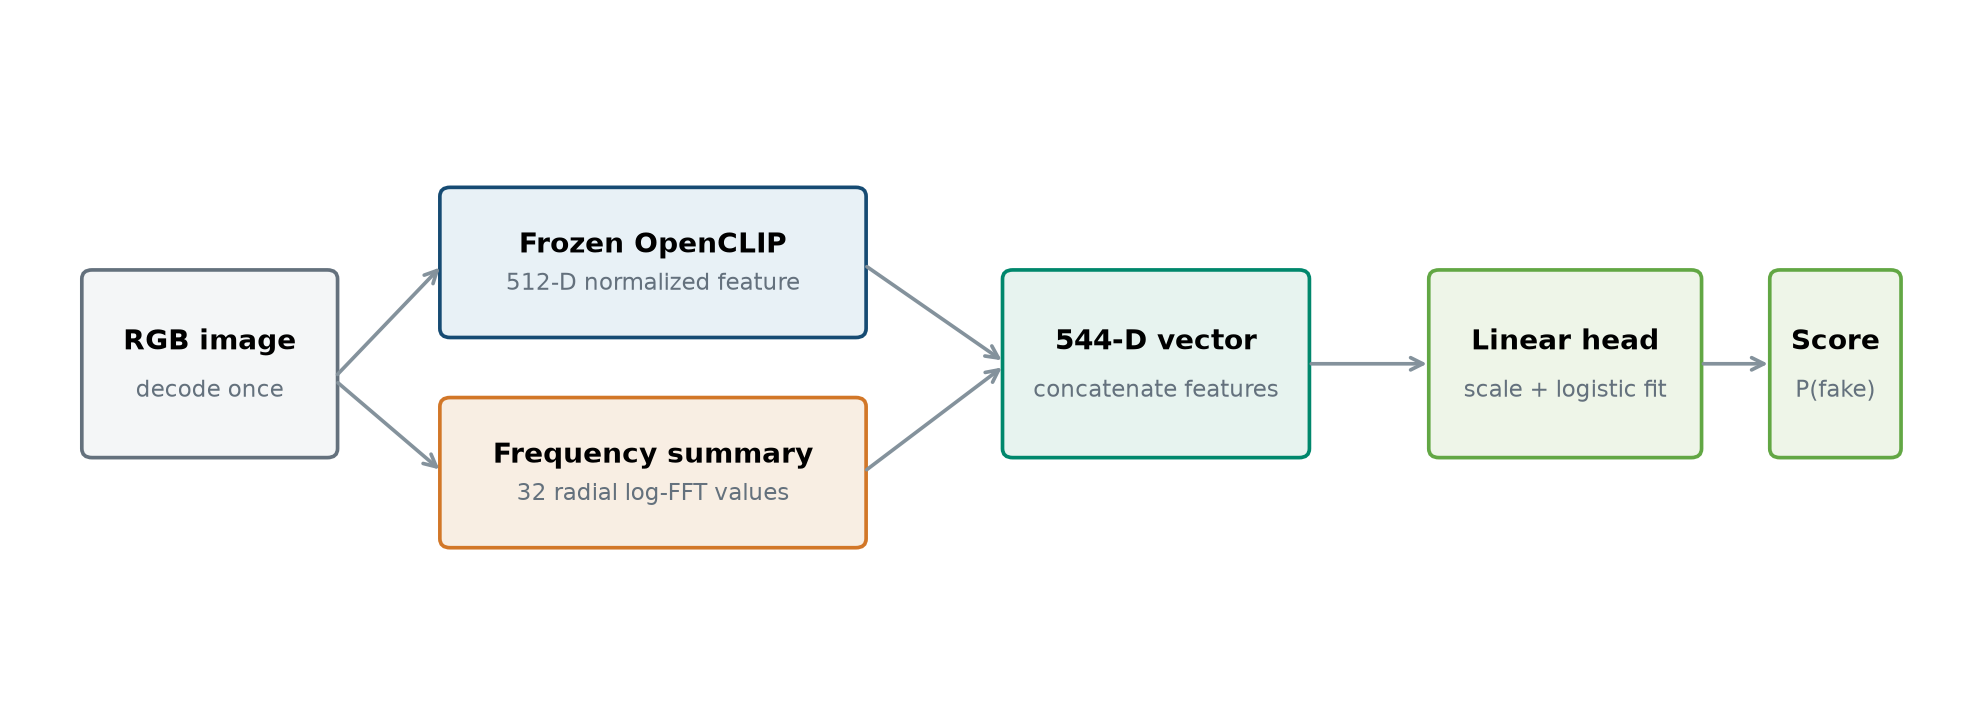
\includegraphics[width=0.98\textwidth]{architecture.png}
  \caption{Feature pipeline for the submitted hybrid detector. The frozen 512-D semantic branch and fixed 32-D
  radial-frequency branch form a 544-D representation. The standardization statistics and logistic head
  are learned; the backbone and frequency descriptor are fixed.}
  \label{fig:architecture}
\end{figure*}

\section{Model Design and Iteration}

\subsection{Task Definition}

Given an RGB image $x$, the detector returns a score $p(x)\in[0,1]$. Larger values rank the image as
more likely to be generated. I use $y=0$ for real and $y=1$ for generated images. ROC AUC is the
primary metric because it evaluates ranking over every threshold; accuracy and F1 are secondary
diagnostics at a selected threshold.

\subsection{Original Hybrid}

Figure~\ref{fig:architecture} shows the submitted design. Each image follows two fixed feature paths.
I concatenate and standardize their outputs before passing them to logistic regression. The
151,277,313 parameters of the OpenCLIP backbone remain frozen.

The semantic branch uses OpenCLIP \code{ViT-B-32-quickgelu} with the \code{openai} checkpoint. If
$f_{\mathrm{CLIP}}(x)\in\mathbb{R}^{512}$ is the image encoder, the stored feature is
\begin{equation}
  s(x)=\frac{f_{\mathrm{CLIP}}(x)}{\lVert f_{\mathrm{CLIP}}(x)\rVert_2}.
\end{equation}
Features are extracted under half-precision autocast, normalized in floating point, cached as
\code{float16}, and promoted to \code{float32} before fitting.

The frequency path converts the image to grayscale, resizes it to $256\times256$, subtracts the mean,
and applies a two-dimensional Hann window before computing
\begin{equation}
  M(u,v)=\log\!\left(1+\left|\mathcal{F}\{x_w\}(u,v)\right|\right).
\end{equation}
After shifting zero frequency to the centre, I divide normalized radius into 32 equal-width bins:
\begin{equation}
 r_k(x)=\frac{1}{|B_k|}\sum_{(u,v)\in B_k}M(u,v),\quad k=1,\ldots,32.
\end{equation}
The descriptor has no learned parameters.

For the hybrid, $z(x)=[s(x);r(x)]\in\mathbb{R}^{544}$. I fit a \code{StandardScaler} on the training
features, followed by L2-regularized logistic regression~\cite{pedregosa2011sklearn}:
\begin{equation}
 p(x)=\sigma\!\left(w^\top\operatorname{std}(z(x))+b\right).
\end{equation}
The interface calls this value \code{P(FAKE)}, but it is not calibrated to deployment prevalence. It
is a confidence score, not proof of a literal real-world probability. For the saturation audit I also
evaluate the pre-sigmoid margin, which preserves ordering when finite-precision probabilities tie.

\subsection{Promoted Semantic Model}

The successor removes $r(x)$ and uses the same scaler-plus-logistic-regression pattern on the 512-D
semantic feature. I balanced its 24,000 source images across CIFAKE, SID-Set, and WildFake, with
4,000 real and 4,000 generated images per domain. Each image contributes one clean view and one
deterministically transformed view, producing 48,000 fitting rows.

For WildFake fitting, I used nine allowed groups: ADM, DDPM, GALIP, GigaGAN, VQGAN, VQVAE, AFHQ,
CelebA-HQ, and LSUN-Church. COCO val2017, DALL-E Advanced, and all frozen evaluation identifiers are
excluded. The threshold, 0.7819586396, was selected on a disjoint 500-real/500-generated SID
calibration split by maximizing Youden's $J=\mathrm{TPR}-\mathrm{FPR}$, with ties resolved toward 0.5.
The final head has 512 coefficients and one intercept.

\section{Data and Evaluation Protocol}

\subsection{CIFAKE and Transformations}

CIFAKE contains $32\times32$ JPEG images derived from CIFAR-10 real images and generated
counterparts~\cite{bird2024cifake}. The published split is preserved: 50,000 real and 50,000 generated
training images, followed by 10,000 real and 10,000 generated test images. Test labels are not used for
fitting. However, I compared model variants on this matrix, so it is development/model-selection
evidence rather than a final untouched test. All 20,000 images are scored under every condition.

I apply transformations individually rather than stacking them. For augmented fitting, family and
severity are selected deterministically from the SHA-256 of the global seed, image identifier, and
transform key. Each image appears once in its clean form and once in a transformed form.

\begin{table}[t]
\centering
\caption{Individual transformation protocol.}
\label{tab:transforms}
\small
\begin{tabularx}{\columnwidth}{@{}lX@{}}
\toprule
Family & Values and implementation \\
\midrule
JPEG & Quality 90, 70, 50, 30; encode/decode, 4:2:0 \\
Blur & $\sigma=0.5,1.0,2.0$; Gaussian blur \\
Resize & $0.5,0.25$; bicubic downsample then restore \\
Noise & $\sigma=0.02,0.05,0.10$; additive RGB noise \\
Jitter & $\pm20\%$ brightness, contrast, saturation \\
Crop & Centre 80\% retained, then bicubic restore \\
\bottomrule
\end{tabularx}
\end{table}

If $A_0$ is clean AUC and $A_j$ is AUC under transformed condition $j$, then
\begin{equation}
 A_{\mathrm{robust}}=\frac{1}{14}\sum_{j=1}^{14}A_j,
 \qquad S=0.5A_0+0.5A_{\mathrm{robust}}.
\end{equation}
For a secondary family-balanced score, I first average within each family and then across the six
families.

\subsection{Frozen Blind Samples}

I froze the original hybrid artifact before selecting three balanced 400-image samples. Each sample
contains 200 real and 200 generated images. The manifests preserve identifiers, paths, labels,
dimensions, byte sizes, and hashes.

SID validation uses label 0 and label 1 images from SID-Set revision \code{dc03ead...}~\cite{sidset}.
WildFake default uses COCO val2017 and DALL-E Advanced; a dimension-matched configuration uses
LAION-5B and DALL-E Advanced~\cite{wildfake}. These sets jointly change generator, real-image source,
content, resolution, and compression history; they do not isolate generator shift. Sampling seeds are
2028, 2026, and 2027. The frozen hybrid SHA-256 is
\code{e9bc59e4...c3427b5e}. Five thousand stratified bootstrap replicates estimate 95\% AUC intervals.

I also audit raw decision margins, exact probability saturation, calibration, simple metadata-only
baselines, and SHA-256 overlap. Twenty deterministic half-samples test sensitivity to sample
composition; they are not independent dataset draws.

\subsection{Promotion Gates}

After the diagnosis, I made these held-out source configurations explicit promotion gates for the
semantic-only successor. Fitting excludes their identifiers, but I used the gates to decide whether
to promote the model. They are strong held-out validation evidence, not a new untouched post-promotion
blind test. A genuinely independent evaluation remains future work. The promoted SHA-256 is
\code{0c1cf7d6...9208449cf}.

\subsection{Compute}

I ran the experiments on Windows 11 with an AMD Ryzen 7 7800X3D, 32 GB RAM, and Radeon RX 7900 XTX
with 24 GB VRAM. The validated stack uses Python 3.12.13, PyTorch 2.9.1 with ROCm 7.2.1, torchvision
0.24.1, OpenCLIP 3.3.0, NumPy, Pillow, and scikit-learn. The final native feature extraction, fit, gate
evaluation, and promotion pipeline completed in 547.063 seconds under a hard 3,600-second budget.

\section{What Worked on CIFAKE}

\subsection{Transformation Robustness}

The original hybrid performed well across most of the challenge matrix. JPEG remained above 0.96 AUC
even at quality 30. Mild blur, moderate resizing, colour jitter, and cropping retained useful ranking.
Quarter-scale resizing and blur at $\sigma=2.0$ were the first conditions below 0.90.

\begin{figure*}[!t]
  \centering
  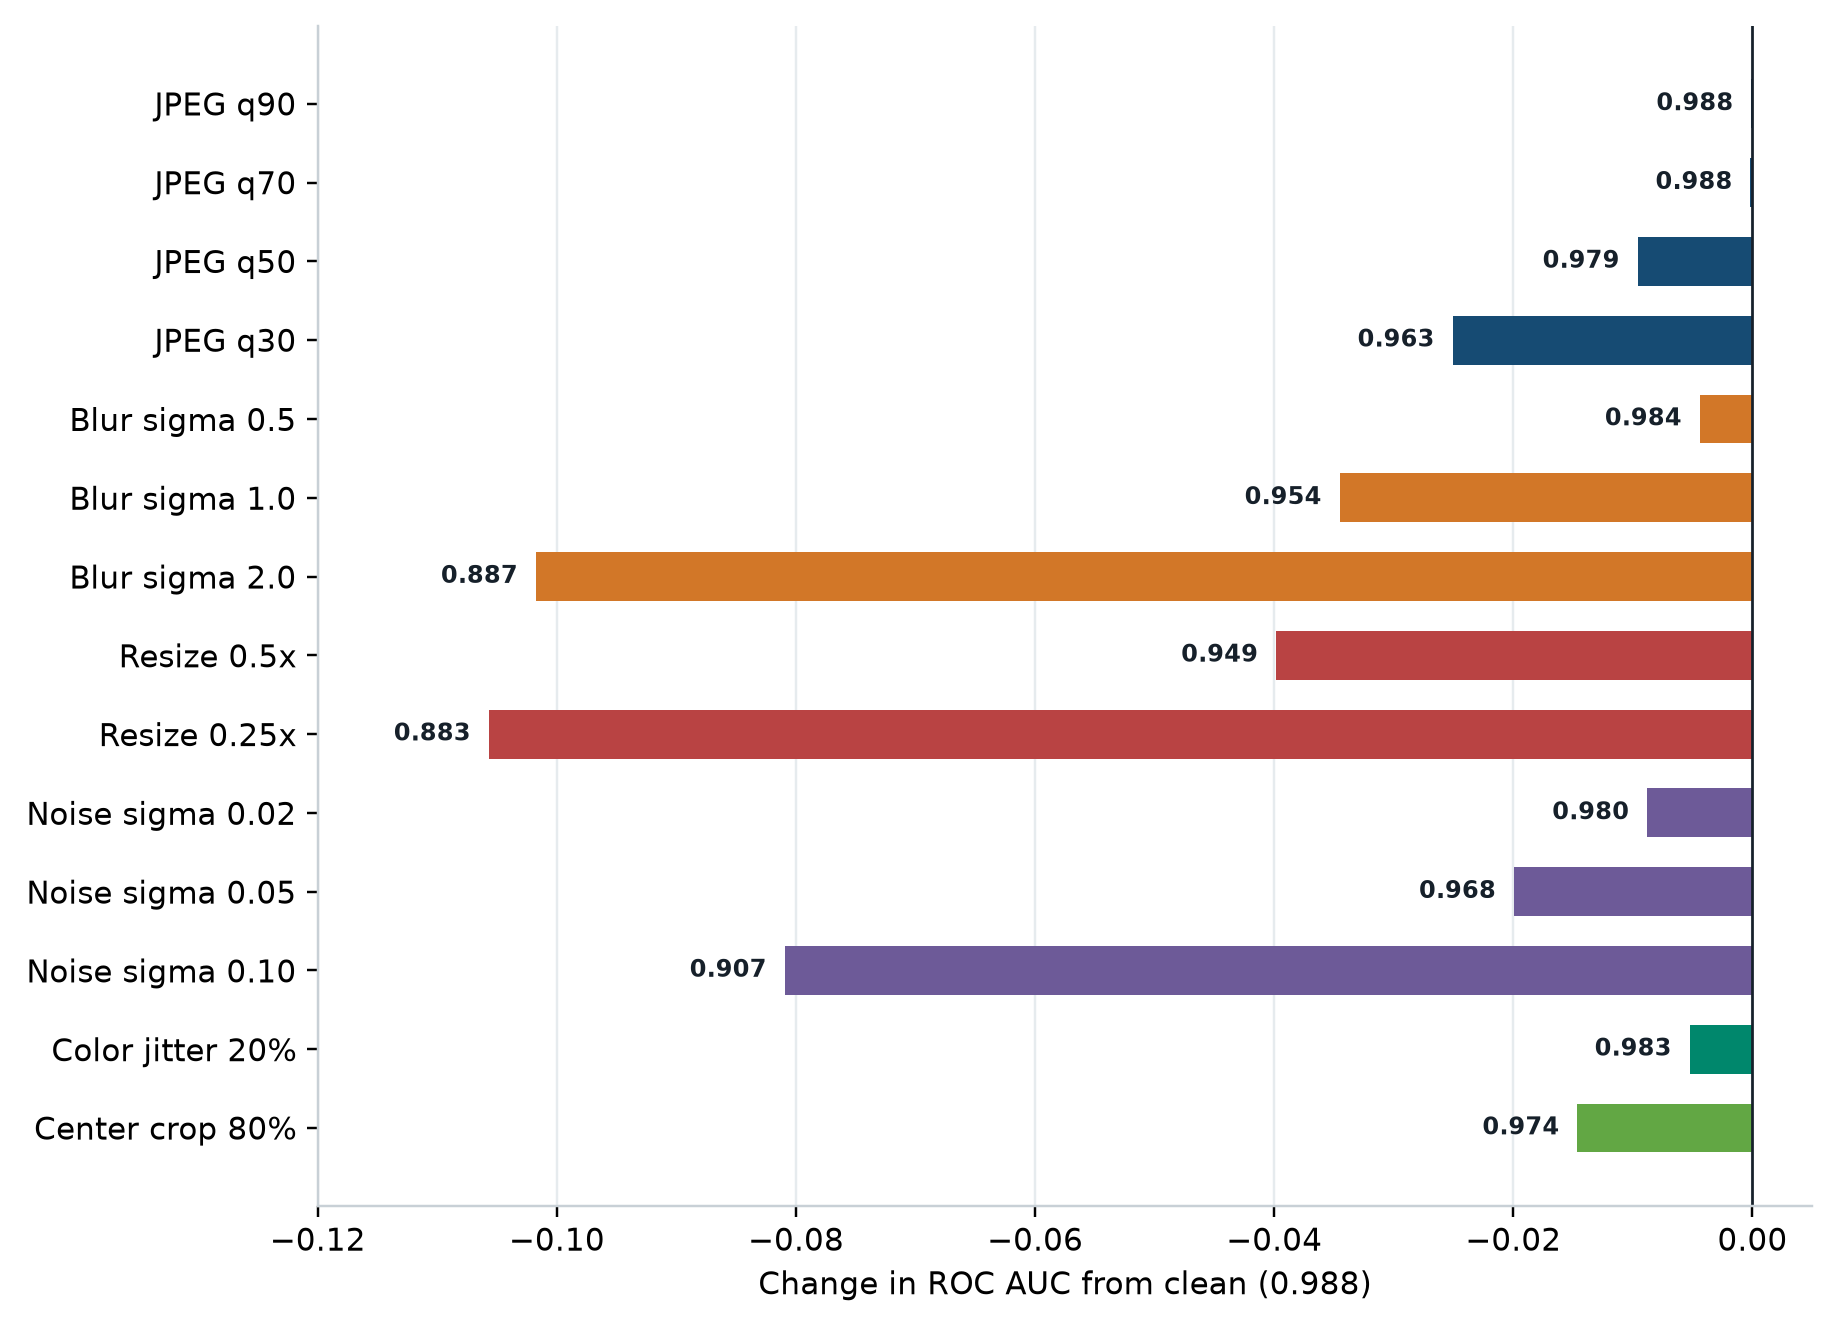
\includegraphics[width=0.98\textwidth]{robustness_conditions.png}
  \caption{ROC AUC for the original hybrid under individual transformations. Every bar uses the same 20,000 held-out CIFAKE
  images. The x-axis reports change from clean performance; labels report absolute AUC.}
  \label{fig:conditions}
\end{figure*}

Figure~\ref{fig:conditions} shows useful robustness to ordinary post-processing until an operation
removes a large amount of image information. It does not, however, test a new generator or source
pipeline.

\subsection{What Supplied the Gain}

The ablation in Table~\ref{tab:ablation} and Figure~\ref{fig:ablation} separates semantic features,
frequency fusion, and augmentation. Adding FFT features raises clean AUC by 0.003005 but lowers robust
AUC by 0.006829. Adding augmentation then lifts robust AUC by 0.045270 relative to the clean hybrid.

\begin{table*}[t]
\centering
\caption{Original CIFAKE ablation. Robust AUC is condition-weighted over 14 transforms.}
\label{tab:ablation}
\small
\begin{tabular}{@{}lccc@{}}
\toprule
Model and fitting data & Clean AUC & Robust AUC & Composite \\
\midrule
Semantic, clean & 0.988755 & 0.917770 & 0.953263 \\
Semantic + FFT, clean & \textbf{0.991760} & 0.910941 & 0.951351 \\
Semantic + FFT, clean + augmented & 0.988409 & \textbf{0.956211} & \textbf{0.972310} \\
\bottomrule
\end{tabular}
\end{table*}

\begin{figure*}[!t]
  \centering
  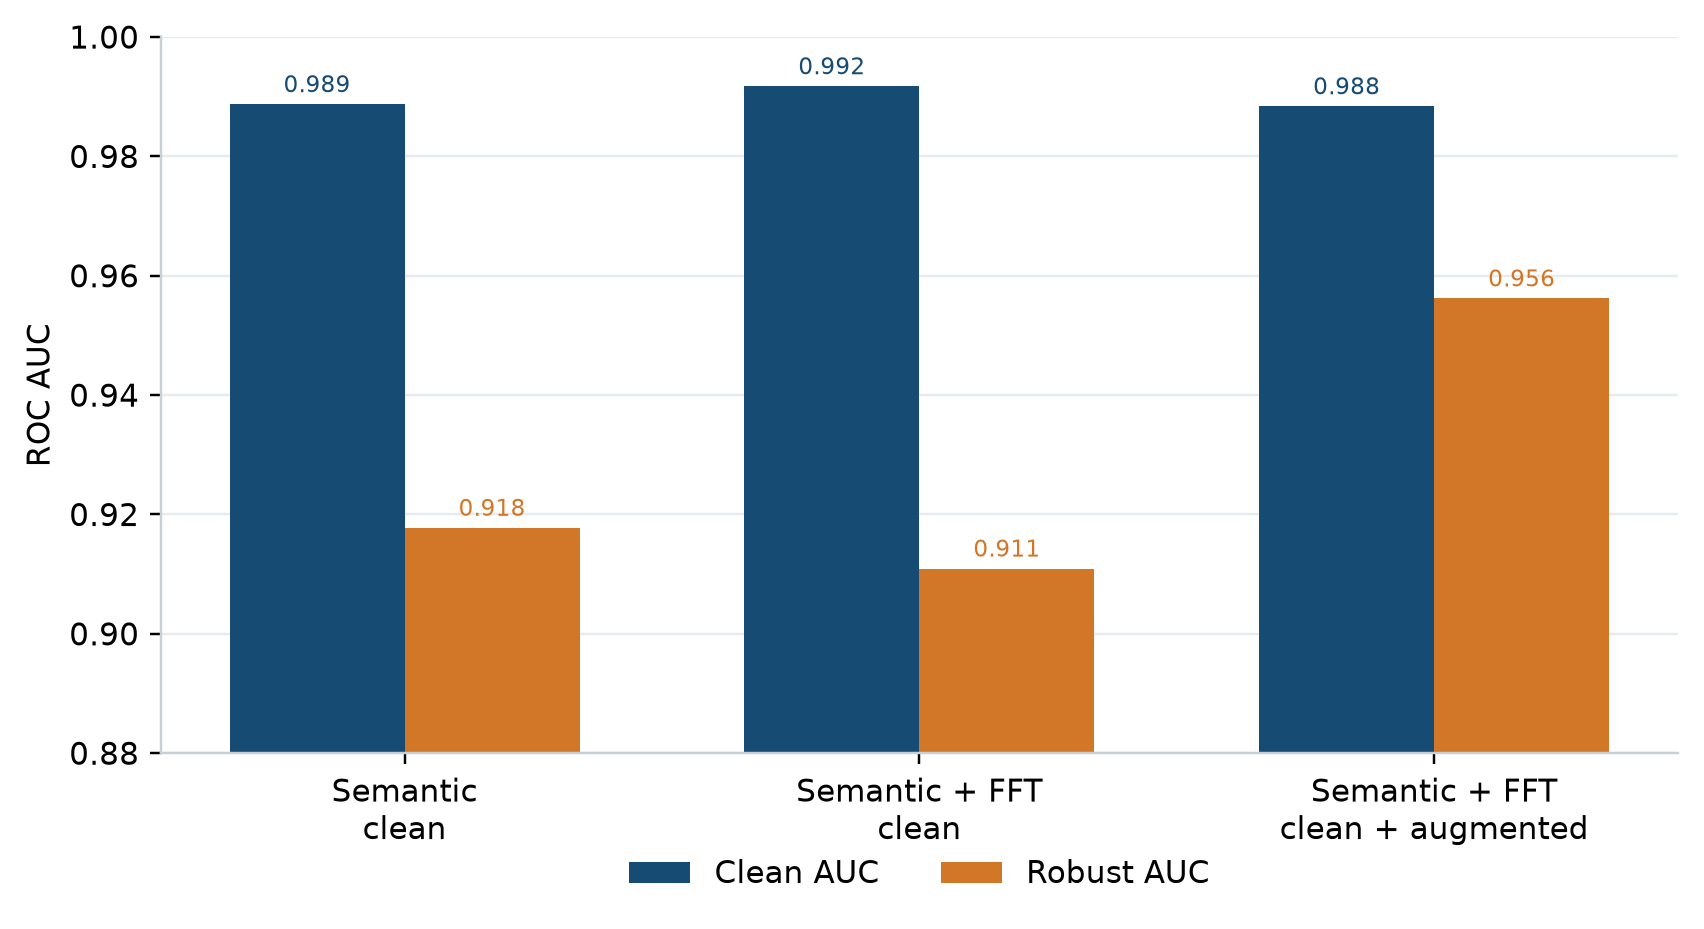
\includegraphics[width=0.93\textwidth]{ablation.png}
  \caption{Clean and robust ROC AUC for three CIFAKE feature and training configurations. Robust AUC is the
  condition-weighted mean over 14 transformations.}
  \label{fig:ablation}
\end{figure*}

The frequency branch alone did not create the robustness gain. The improvement appeared after the
hybrid saw deterministic transformations during training.

\subsection{Benchmark Trade-Off}

The promoted semantic model is not a free improvement: it gives up some CIFAKE performance in exchange
for substantially better native-resolution transfer.

\begin{table}[H]
\centering
\caption{CIFAKE trade-off between artifact stages.}
\label{tab:tradeoff}
\small
\begin{tabularx}{\columnwidth}{@{}Xccc@{}}
\toprule
Artifact stage & Clean & Robust & Composite \\
\midrule
Original hybrid & \textbf{.988409} & \textbf{.956211} & \textbf{.972310} \\
Promoted semantic & .957820 & .896636 & .927228 \\
\bottomrule
\end{tabularx}
\end{table}

For the promoted model, the hardest CIFAKE conditions are blur $\sigma=2.0$ at 0.785540 AUC, resize
0.25 at 0.774426, and noise $\sigma=0.10$ at 0.797451. This trade-off is important and should not be
hidden behind the stronger native-domain numbers.

\section{Where the Hybrid Failed}

\subsection{Blind Probabilities Collapsed}

The blind result is the turning point because it overturns the benchmark selection. The semantic
baseline retains ranking information on all three samples. Both hybrids emit severely saturated
probabilities, and the selected augmented hybrid calls every image fake at threshold 0.5.

\begin{figure*}[!t]
  \centering
  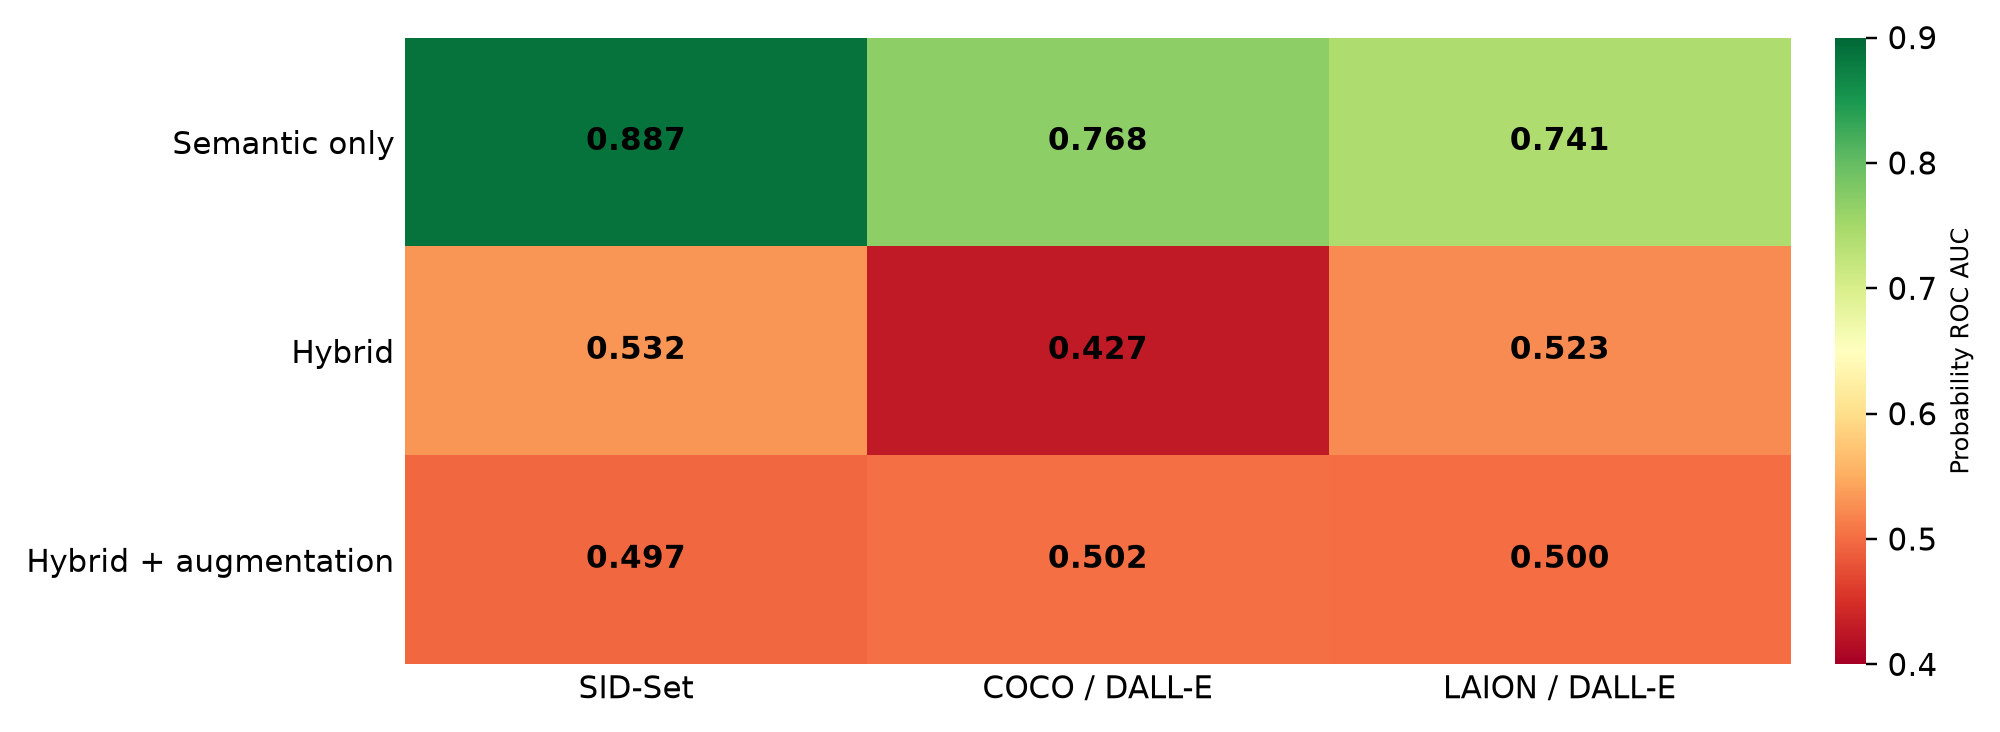
\includegraphics[width=0.96\textwidth]{blind_transfer.png}
  \caption{Probability ROC AUC on three frozen, balanced native-resolution samples for the three model
  variants. Each cell uses the same 200-real/200-generated sample; raw-margin results follow in
  Table~\ref{tab:margin}.}
  \label{fig:blind}
\end{figure*}

\begin{table*}[t]
\centering
\caption{Blind probability ROC AUC by frozen model variant.}
\label{tab:blind}
\small
\begin{tabular}{@{}lccc@{}}
\toprule
Frozen model & SID-Set & COCO / DALL-E & LAION / DALL-E \\
\midrule
Semantic & \textbf{0.886975} & \textbf{0.767975} & \textbf{0.740600} \\
Hybrid & 0.532475 & 0.427500 & 0.523488 \\
Hybrid + augmentation & 0.497500 & 0.502500 & 0.500000 \\
\bottomrule
\end{tabular}
\end{table*}

The default WildFake sample has an obvious image-size association, but the failure remains in the
LAION dimension-matched configuration, where size-only AUC is 0.5. Resolution mismatch alone therefore does not
explain the collapse.

\begin{table*}[t]
\centering
\caption{Selected hybrid probability and raw-margin AUC. Intervals are 5,000-replicate stratified
bootstrap 95\% intervals. ``Exact 1'' counts emitted probabilities equal to 1.0.}
\label{tab:margin}
\small
\begin{tabular}{@{}lccc@{}}
\toprule
Blind set & Probability AUC [95\% CI] & Margin AUC [95\% CI] & Exact 1 \\
\midrule
SID-Set & .4975 [.4925, .5000] & .7598 [.7114, .8034] & 399/400 \\
COCO / DALL-E & .5025 [.5000, .5075] & .5377 [.4797, .5942] & 399/400 \\
LAION / DALL-E & .5000 [.5000, .5000] & .7140 [.6629, .7630] & 400/400 \\
\bottomrule
\end{tabular}
\end{table*}

\subsection{Frequency Extrapolation}

The branch-level values provide a concrete mechanism. I fitted the original frequency standardization
recipe on 200,000 clean-plus-augmented training rows. The training 99.9th percentile of absolute
standardized frequency values is 5.48, the training maximum is 15.34, and the clean CIFAKE test maximum
is 12.15.

The blind maxima are 507.99 on SID-Set, 498.14 on COCO/DALL-E, and 505.87 on LAION/DALL-E. On SID,
total hybrid logits range from 7.96 to 121.44. Since $\sigma(7.96)\approx0.99965$, even the minimum is
already close to one.

\begin{figure*}[!t]
  \centering
  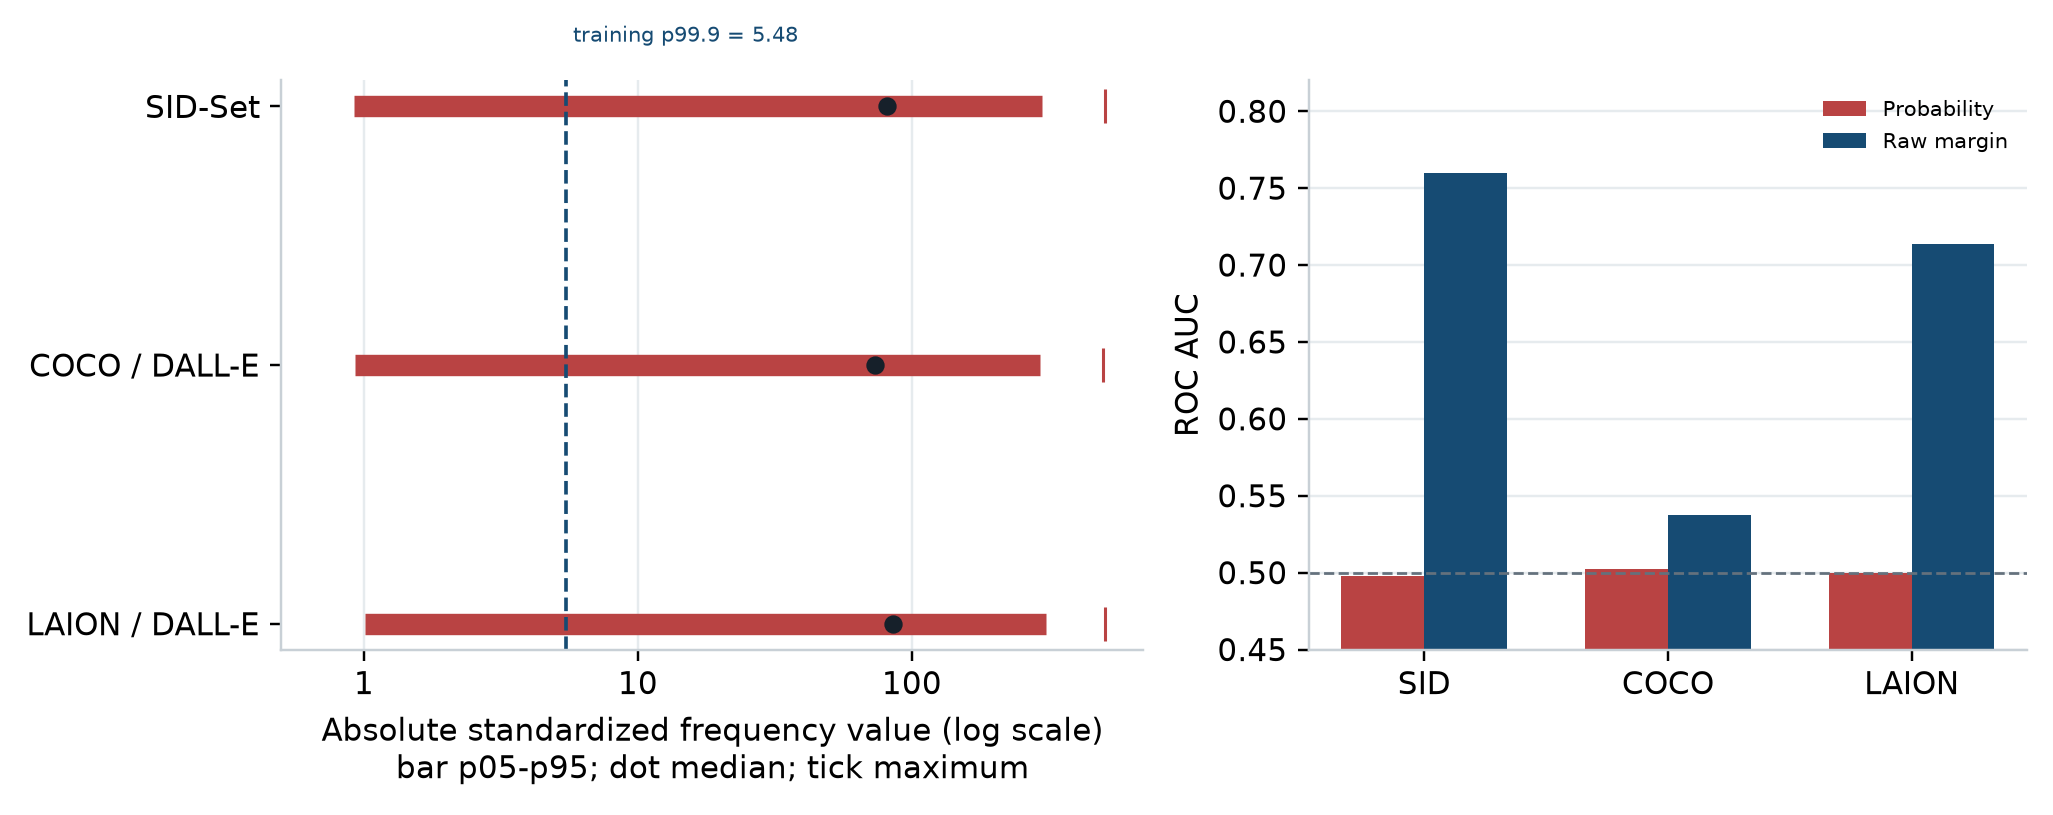
\includegraphics[width=0.98\textwidth]{frequency_extrapolation.png}
  \caption{Frequency-branch diagnosis. The left panel compares the maximum absolute standardized value on
  clean and blind inputs; the right panel lists the resulting range shift through the linear head.}
  \label{fig:frequency}
\end{figure*}

These values explain why threshold metrics and probability AUC collapse. Changing a threshold on the
rounded probabilities cannot separate hundreds of ties. The raw margins reveal a more precise result:
ranking survives on SID and LAION/DALL-E, but is weak and statistically compatible with chance on
COCO/DALL-E. The defect is therefore an unusable public score plus unstable transfer, not uniform
destruction of ranking. Blind maxima are about $42\times$ the clean-CIFAKE maximum and about
$93\times$ the training 99.9th percentile.

The audit also exposes dataset shortcuts. Five-fold metadata-only probes using width, height, byte
size, and aspect ratio reach mean AUCs of 0.971 on SID, 1.000 on COCO/DALL-E, and 0.643 on
LAION/DALL-E. This does not prove that the image model uses those fields, but it shows that labels and
source pipelines are confounded. Exact SHA-256 screening finds no fitting/evaluation overlap; the
LAION/DALL-E manifest contains five repeated files. A difference-hash screen flags a few candidates,
including one cross-label match, so it is treated as a warning rather than proof of duplication.

\section{Remediation and Promotion}

Before replacing \code{outputs/model.joblib}, I required the semantic-only successor to pass every
recorded gate.

\begin{table}[H]
\centering
\caption{Promoted semantic-only gates. PFR is predicted fake rate at threshold 0.7819586396.}
\label{tab:gates}
\small
\begin{tabularx}{\columnwidth}{@{}Xccc@{}}
\toprule
Gate & ROC AUC & PFR & Result \\
\midrule
SID calibration & 0.993972 & 0.5130 & Pass \\
SID validation & 0.991900 & 0.5075 & Pass \\
COCO / DALL-E & 0.902925 & 0.5275 & Pass \\
LAION / DALL-E & 0.912700 & 0.4050 & Pass \\
\bottomrule
\end{tabularx}
\end{table}

The successor removes the observed saturation and improves held-out ranking. On SID its confusion
counts are TN/FP/FN/TP $=189/11/8/192$; on COCO/DALL-E they are $162/38/27/173$; and on
LAION/DALL-E they are $183/17/55/145$. Corresponding 95\% AUC intervals are [.9856, .9967],
[.8717, .9300], and [.8822, .9400]. Balanced-sample Brier scores are .049, .152, and .124, so the
confidence values still should not be interpreted as deployment probabilities. This does not prove
universal generalisation. Because these datasets influenced promotion, the next credible test must use
generators and sources that were not used for fitting, calibration, or model selection.

\begin{table}[t]
\centering
\caption{Promoted model under native-resolution transformations. The individual column is mean
(minimum) AUC across 14 conditions.}
\label{tab:native-stress}
\small
\begin{tabular}{@{}lccc@{}}
\toprule
Set & Clean & Individual & Chains \\
\midrule
SID & .992 & .980 (.946) & .975 \\
COCO / DALL-E & .903 & .864 (.735) & .771 \\
LAION / DALL-E & .913 & .907 (.862) & .914 \\
\bottomrule
\end{tabular}
\end{table}

I additionally applied all 14 individual transforms to each native sample. Three heuristic
multi-operation re-upload chains combine resize, recompression, colour change, sharpening, and either
crop or noise. They are stress tests, not measurements of a proprietary TikTok processing pipeline.

\begin{figure*}[!t]
  \centering
  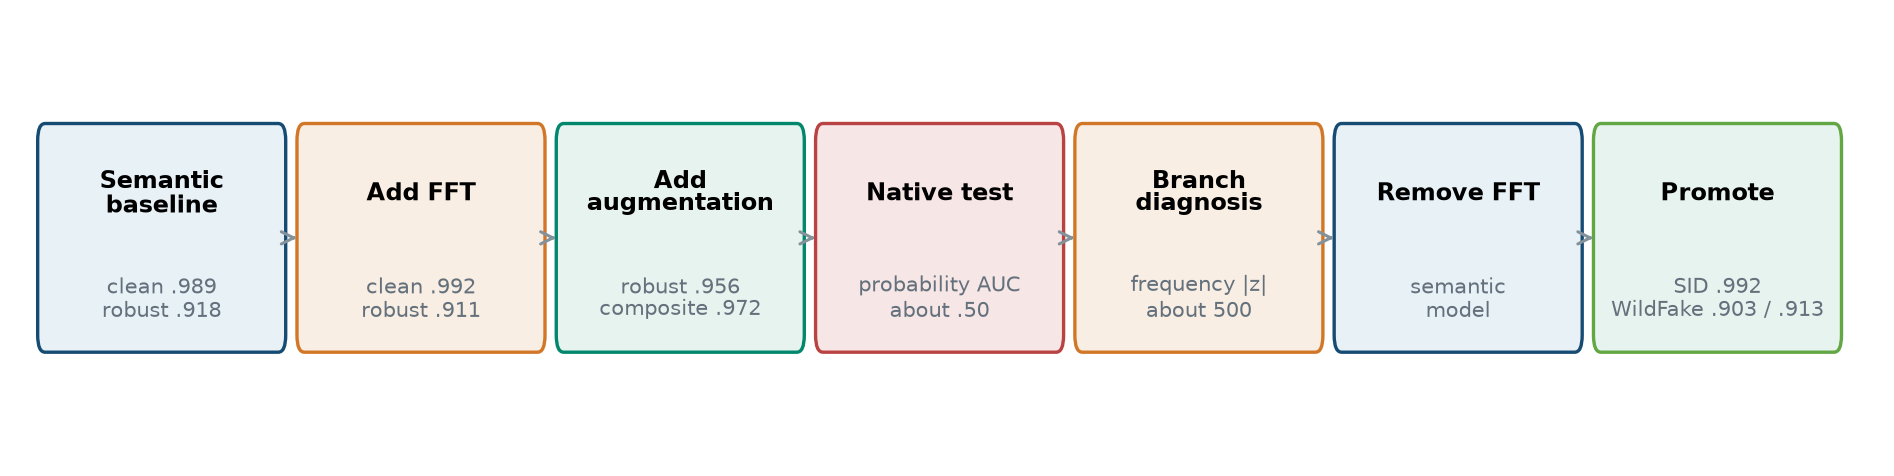
\includegraphics[width=0.98\textwidth]{project_progression.png}
  \caption{Model variants and evaluation steps used during development, from the semantic baseline through
  hybrid training, native-resolution evaluation, branch diagnosis, and semantic-only promotion.}
  \label{fig:progression}
\end{figure*}

Figure~\ref{fig:progression} summarises the iteration. The practical conclusions are clear. Augmentation
is local: training on known transformations teaches useful invariance around CIFAKE, not automatic
invariance to a different generator or source. Plausible features can become shortcuts; unconstrained
linear contributions are dangerous when standardized values leave the fitting range. Finally, model
selection defines what ``best'' means. The CIFAKE composite selected the right model for that matrix
and the wrong model for broad transfer.

\section{Limitations and Responsible Use}

CIFAKE is low-resolution and generator-narrow; its transformed test set still shares the same
underlying dataset and was used for model comparison. The original blind samples and current gates
contain only 400 images each. I used
the native-resolution gates to select the promoted model, so they are no longer an untouched final
test. WildFake fitting covers nine groups, but many generators, editing systems, styles, and capture
pipelines remain unseen.

The native chain tests cover only three hand-specified sequences. Scores are not calibrated to
deployment prevalence.
Demographic bias, adversarial attacks, partial edits, mixed real/generated images, and fairness were
not evaluated. OpenCLIP may inherit biases from pretraining.

This detector is a research prototype. It should not be the sole basis for content removal, account
suspension, copyright decisions, fraud allegations, academic penalties, or authorship claims. False
positives can harm legitimate creators; false negatives can create false confidence. Human review,
provenance metadata, source verification, and multiple independent signals remain necessary.

\caution{The promotion gates are strong held-out evidence, but not a fresh post-promotion blind test.
The next version needs an independent generator-and-source evaluation.}

\section{Reproducibility}

The judge-facing prediction contract for my CLI is:
\begin{quote}\small
\code{python src/predict.py --input\_dir images --out preds.json --device auto}
\end{quote}
The CLI recursively finds JPEG, PNG, and WebP inputs and produces deterministic records containing
\code{image\_path} and continuous \code{pred}. The artifact validates its schema and feature
configuration and rejects non-finite predictions.

I froze both stages, their hashes, plotted values, and provenance in the report snapshot
\code{docs/report\_metrics.json}. This prevents later promotion runs from silently rewriting historical
figures. I rebuild all six figures and the PDF with:
\begin{quote}\small
\code{powershell -ExecutionPolicy Bypass -File scripts/build\_technical\_report.ps1}
\end{quote}
The figure script uses Pillow and repository data rather than downloaded illustrations.

\section{Conclusion}

The original hybrid solved the problem I selected it to solve. Deterministic augmentation raised its
mean transformed CIFAKE AUC to 0.956211 and composite to 0.972310. The frequency branch alone did not
produce that gain.

Blind testing then showed that the selected model did not provide a usable score under compound
domain shift: every image was classified fake and almost every probability rounded to one. Raw-margin
AUC recovered to .760 on SID and .714 on LAION/DALL-E, but remained .538 on COCO/DALL-E. Frequency
features roughly $42\times$ beyond the clean-CIFAKE maximum explained the numerical saturation.

Removing that branch and fitting a semantic-only probe on balanced, multi-domain data produced a
better promotion candidate. The candidate passed the recorded SID and WildFake gates, although its CIFAKE
composite fell to 0.927228. This is an engineering trade-off, not a contradiction.

My next step is an independent post-promotion evaluation on generators and source pipelines that did
not influence fitting, calibration, or gating. Until then, the strongest supported claim is narrow but
useful: transformation robustness and compound domain transfer must be measured separately, and
branch-level out-of-distribution checks can prevent a strong benchmark score from promoting a brittle
model.

\begin{thebibliography}{11}
\small

\bibitem{techjam2026}
TikTok TechJam 2026.
\newblock Robust detection of AI-generated images under real-world transformations.
\newblock Track 5 problem statement and technical workshop notes, 2026.

\bibitem{wang2020cnn}
S.-Y. Wang, O. Wang, R. Zhang, A. Owens, and A. A. Efros.
\newblock CNN-generated images are surprisingly easy to spot... for now.
\newblock In \emph{Proceedings of CVPR}, 2020.
\newblock \url{https://arxiv.org/abs/1912.11035}.

\bibitem{frank2020frequency}
J. Frank, T. Eisenhofer, L. Sch\"onherr, A. Fischer, D. Kolossa, and T. Holz.
\newblock Leveraging frequency analysis for deep fake image recognition.
\newblock In \emph{Proceedings of ICML}, 2020.
\newblock \url{https://arxiv.org/abs/2003.08685}.

\bibitem{ojha2023universal}
U. Ojha, Y. Li, and Y. J. Lee.
\newblock Towards universal fake image detectors that generalize across generative models.
\newblock In \emph{Proceedings of CVPR}, 2023.
\newblock \url{https://arxiv.org/abs/2302.10174}.

\bibitem{zhong2024patchcraft}
N. Zhong, Y. Xu, S. Li, Z. Qian, and X. Zhang.
\newblock PatchCraft: Exploring texture patch for efficient AI-generated image detection.
\newblock arXiv:2311.12397v3, 2024.
\newblock \url{https://arxiv.org/abs/2311.12397}.

\bibitem{poletti2026xai}
S. Poletti, J. Ilyes, M. Hasenbalg, D. Fischinger, and M. Boyer.
\newblock AI-generated images: What humans and machines see when they look at the same image.
\newblock arXiv:2605.06143, 2026.
\newblock \url{https://arxiv.org/abs/2605.06143}.

\bibitem{bird2024cifake}
J. J. Bird and A. Lotfi.
\newblock CIFAKE: Image classification and explainable identification of AI-generated synthetic
images.
\newblock \emph{IEEE Access}, 12:15642--15650, 2024.
\newblock \url{https://doi.org/10.1109/ACCESS.2024.3356122}.

\bibitem{radford2021clip}
A. Radford et al.
\newblock Learning transferable visual models from natural language supervision.
\newblock In \emph{Proceedings of ICML}, 2021.
\newblock \url{https://arxiv.org/abs/2103.00020}.

\bibitem{pedregosa2011sklearn}
F. Pedregosa et al.
\newblock Scikit-learn: Machine learning in Python.
\newblock \emph{Journal of Machine Learning Research}, 12:2825--2830, 2011.

\bibitem{openai2021clip}
OpenAI.
\newblock CLIP: Connecting text and images.
\newblock 5 January 2021. \url{https://openai.com/index/clip/}.

\bibitem{sidset}
SID-Set.
\newblock Hugging Face dataset repository, revision
\code{dc03ead57929879319ce30a82bfcfb8d317b10bd}.
\newblock \url{https://huggingface.co/datasets/saberzl/SID_Set}.

\bibitem{wildfake}
WildFake.
\newblock ModelScope dataset repository and TechJam evaluation subset.
\newblock \url{https://modelscope.cn/datasets/hy2628982280/WildFake/summary}.

\end{thebibliography}

\appendix
\section{Claim-to-Artifact Map}

\small
\noindent\textbf{Original benchmark metrics.}
\path{outputs/clean_metrics.json}; frozen historical conditions in
\path{docs/report_metrics.json}.

\noindent\textbf{Frozen blind evaluation.}
\path{outputs/cross_domain_summary.json}; branch diagnostics in
\path{data/blind-test/ablation_results.json}; margin, uncertainty, calibration, metadata, and overlap
audit in \path{outputs/shift_audit.json}.

\noindent\textbf{Promoted model.}
Training recipe and gates in \path{outputs/native_metrics.json}; per-condition results in
\path{outputs/robustness_table.csv}; wall-clock stages in
\path{outputs/native_training_timing.json}; native individual and chained stress tests in
\path{outputs/native_stress.json}.

\noindent\textbf{Inference and report provenance.}
\path{src/predict.py}; immutable plotted values and recipes in
\path{docs/report_metrics.json}.

\end{document}
